\documentclass[conference]{IEEEtran}
% Needed so that \thanks can be used in \author for the funding footnote.
\IEEEoverridecommandlockouts
% English submission version. Compile with XeLaTeX (see build.sh).
% IEEE requires Times; under XeLaTeX, IEEEtran's Times fallback must be
% replaced explicitly or the body would silently render in Latin Modern.
\usepackage{fontspec}
\setmainfont{Times New Roman}
\setsansfont{Arial}
\setmonofont{Courier New}

\usepackage{cite}
\usepackage{amsmath,amssymb,amsfonts}
\usepackage{graphicx}
\usepackage{booktabs}
\usepackage{array}
\usepackage{textcomp}
\usepackage{xcolor}
\usepackage{url}

\graphicspath{{../../figures/generated/}}

% IEEEtran's conference \and does not create a tabular column: it ends one
% halign and starts another, joining the blocks with stretchy \hfill. Each row
% then distributes its leftover space independently, so the author blocks land
% at different x offsets from row to row. Building the block as a real tabular
% instead makes the columns genuinely shared across rows, which keeps every
% author centred under the one above it.
\makeatletter
\newcommand{\authname}[1]{{\@IEEEauthorblockNstyle #1}}
\newcommand{\authaff}[1]{{\@IEEEauthorblockAstyle #1}}
\makeatother

\begin{document}

\title{Dynamic Graph Neural Policies for Multi-Robot Cooperative
Navigation: Edge Features, Safety Filtering, and Density Limits}

\author{%
\begin{tabular}{@{}*{3}{>{\centering\arraybackslash}p{0.31\textwidth}}@{}}
\authname{Xuelin Hu} & \authname{Xiaoqin Fu} & \authname{Youjing Fu} \\[0.9ex]
\authaff{\textit{Liuzhou Railway Vocational}} &
\authaff{\textit{Liuzhou Railway Vocational}} &
\authaff{\textit{College of Earth and}} \\
\authaff{\textit{Technical College}} & \authaff{\textit{Technical College}} &
\authaff{\textit{Environmental Sciences}} \\
 & & \authaff{\textit{Lanzhou University}} \\
\authaff{Liuzhou 545000, China} & \authaff{Liuzhou 545000, China} &
\authaff{Lanzhou 730000, China} \\
\authaff{huxl@ltzy.edu.cn} & \authaff{fuxiaoqin@ltzy.edu.cn} &
\authaff{fuyj2025@lzu.edu.cn} \\[2.2ex]
\authname{Jingchao Wang\textsuperscript{*}} & \authname{Pengming Hu} & \authname{Simeng Li} \\[0.9ex]
\authaff{\textit{School of Computer Science}} &
\authaff{\textit{School of Computer Science}} &
\authaff{\textit{Liuzhou Railway Vocational}} \\
\authaff{\textit{Zhongyuan University}} &
\authaff{\textit{Zhongyuan University}} &
\authaff{\textit{Technical College}} \\
\authaff{\textit{of Technology}} & \authaff{\textit{of Technology}} & \\
\authaff{Zhengzhou 450007, China} & \authaff{Zhengzhou 450007, China} &
\authaff{Liuzhou 545000, China} \\
\authaff{static@zut.edu.cn} & \authaff{hupengming@zut.edu.cn} &
\authaff{lisimeng@ltzy.edu.cn}
\end{tabular}%
\thanks{This work was supported by the Science and Technology Research
Project of Henan Province (grant no.~262102211055) and the Key Scientific
Research Project of Colleges and Universities in Henan Province (grant
no.~27AQ520018).}
\thanks{\textsuperscript{*}Corresponding author: Jingchao Wang.}
}

\maketitle

\begin{abstract}
Multi-robot navigation requires coordinated motion and collision avoidance
under changing neighbor relations and limited communication. This paper
presents a dynamic graph neural policy that represents robots as nodes and
local communication links as edges. Five-dimensional relative-motion edge
features encode relative position, velocity, and closing speed, while shared
message passing produces local velocity commands for variable-size teams.
The policy is trained by imitation with separation, goal-progress, and
smoothness losses, and an external safety filter corrects approaching robot
pairs during execution. Evaluation covers four map families and teams of
5--40 robots, with 30 unseen seeds per multi-scale configuration. Local
message passing improves goal-reaching success over an edge-free policy of
the same capacity. Safety filtering reduces close encounters and increases
minimum inter-robot separation. In the tested 5--10-robot settings, the
filtered policies achieve high collision-free success while retaining
millisecond-level control time. These results support the use of local graph
interaction and safety filtering for cooperative navigation at low to
moderate team densities.
\end{abstract}

\begin{IEEEkeywords}
multi-robot systems, graph neural networks, cooperative navigation, collision
avoidance, dynamic interaction graphs.
\end{IEEEkeywords}

\section{Introduction}

Multi-robot cooperative navigation requires robots to reach assigned goals
without colliding with one another or with static obstacles. As the number
of robots increases, joint planning becomes more costly and local
interactions become harder to coordinate. These interactions also change as
neighbors enter and leave sensing range. Centralized search must account for
the joint state space, whereas independent policies do not explicitly model
the relationships among robots.

Graph neural networks (GNNs) represent these relationships through robot
nodes and communication edges. Message passing aggregates neighbor
information, and parameter sharing allows the same policy to process
different team sizes. Rebuilding edges from current positions updates the
interaction structure as the robots move.

We examine how local graph communication affects goal-reaching success
relative to a policy using only its own node features. We also evaluate how
communication radius and safety filtering affect collision risk and control
time. Comparisons use the same observations, action limits, and termination
rules.

Our contributions are:
\begin{itemize}
  \item a dynamic graph policy using five-dimensional edge features for
  normalized relative position, relative velocity, and closing speed, with
  shared message passing for variable-size robot teams;
  \item a training and execution scheme combining action imitation,
  one-step separation, goal progress, and smoothness losses with an optional
  external pairwise safety filter, whose effect is evaluated separately from
  the neural policy;
  \item a reproducible evaluation across four map families, 5--40 robots, and
  30 unseen seeds, with classical and neural baselines and graph, radius, and
  safety ablations to measure the effects of robot density.
\end{itemize}

\section{Related Work}

\subsection{Classical and Rule-Based Planning}
A* uses heuristic search to find paths on a discretized map
\cite{hart1968}. In multi-robot settings, independently planned paths still
require coordination to avoid conflicts. Velocity-obstacle methods identify
velocities that would lead to collisions under predicted relative motion
\cite{fiorini1998}. Their geometric formulation supports local collision
avoidance, with performance depending on the prediction horizon and the
assumptions about neighboring agents' motion.

\subsection{Learned Multi-Robot Collision Avoidance}
Decentralized deep reinforcement learning maps local observations to motion
commands, reducing the need for joint planning
\cite{long2018orcamarl, thumiger2022uav}. Curriculum learning introduces
increasingly difficult constrained passages \cite{komol2025curriculum};
physics-informed priors guide policy learning \cite{feng2024physics}; and
semi-supervised methods reduce labeling requirements
\cite{parooei2023semisupervised}. Related studies address communication and
formation constraints in vessel navigation \cite{niu2023ship, wang2025ships}.

\subsection{Graph Representations for Robot Teams}
Diao \textit{et al.} encode spatial relations with a GNN for path planning
\cite{diao2024gnn}. He \textit{et al.} combine graph attention with
hierarchical motion planning to weight neighboring agents
\cite{he2023ganav}. Goarin and Loianno use a GNN for decentralized goal
assignment \cite{goarin2024assignment}, while Yang \textit{et al.} combine
a GNN with PPO for multi-UAV planning \cite{yang2025uav}. A recent survey
reviews rule-based and learned coordination methods for multi-robot
collision avoidance \cite{yang2025survey}.

This work combines a graph policy for local motion with a separate filter
for approaching robot pairs. Graph and filter ablations distinguish the
effects of learned interaction from those of action correction. Tests across
four map families and five team sizes assess how these effects change with
robot density.

\section{Problem Formulation}

Let $\mathcal{V}=\{1,\dots,N\}$ index the robots, with position
$p_i\in\mathbb{R}^2$, velocity $v_i\in\mathbb{R}^2$, and goal
$g_i\in\mathbb{R}^2$. A directed communication graph is rebuilt at every step
from a radius $R_c$:
\begin{equation}
A_{ij}=
\begin{cases}
1, & i\neq j,\ \|p_i-p_j\|\le R_c,\\
0, & \text{otherwise.}
\end{cases}
\end{equation}

Node features are eight-dimensional: goal-relative position, normalized
velocity, direction and distance to the nearest obstacle, and a bias term. The
policy emits a two-dimensional local velocity $u_i$ with
$\|u_i\|\le v_{\max}=1.4$~m/s, and positions evolve as
$p_i^{t+1}=p_i^t+\Delta t\,u_i^t$ with $\Delta t=0.08$~s.

We distinguish safety-distance violations from physical collisions. A
\emph{safety violation} occurs when a pair is closer than $d_s=0.72$~m; a
\emph{physical collision} occurs when the distance is less than the sum of
the robot radii, $0.56$~m. An event is counted when a pair crosses from outside
to inside the corresponding threshold; a sustained violation counts as one
event. Task success requires the final mean goal error across all robots to
fall below a fixed threshold. Strict collision-free success additionally
requires that no physical collision occur during the episode.

Relative position and velocity are normalized by map size and maximum speed,
respectively. For a directed edge $(j,i)$, the five-dimensional feature is
\begin{equation}
e_{ij}^t=\left[\frac{p_i^t-p_j^t}{[W,H]},\ \frac{v_i^t-v_j^t}{v_{\max}},\
\frac{-\big((v_i^t-v_j^t)\cdot\hat{r}_{ij}^t\big)}{v_{\max}}\right],
\end{equation}
with $\hat{r}_{ij}^t=(p_i^t-p_j^t)/(\|p_i^t-p_j^t\|+\epsilon)$ and $[W,H]$ the
map extents. The closing-speed component is positive when the robots
approach each other, providing information about relative motion in
addition to distance.

\section{Method}

\subsection{System Overview}
Fig.~\ref{fig:arch} organizes the closed loop from left to right: the robot
scene and observed states, structured graph inputs, feature embedding, the
shared GNN policy, and velocity output with optional safety filtering.
Each robot supplies an eight-dimensional node feature; communication-radius
edges carry five-dimensional relative-motion features. The shared encoder
and three message-passing layers produce node representations for a shared
two-dimensional velocity head. Executed actions update the scene and the
graph is rebuilt at the next control step. Candidate actions illustrate
motion choices; the learned policy directly regresses velocity rather than
receiving a candidate-action list as input.

\begin{figure*}[t]
\centering
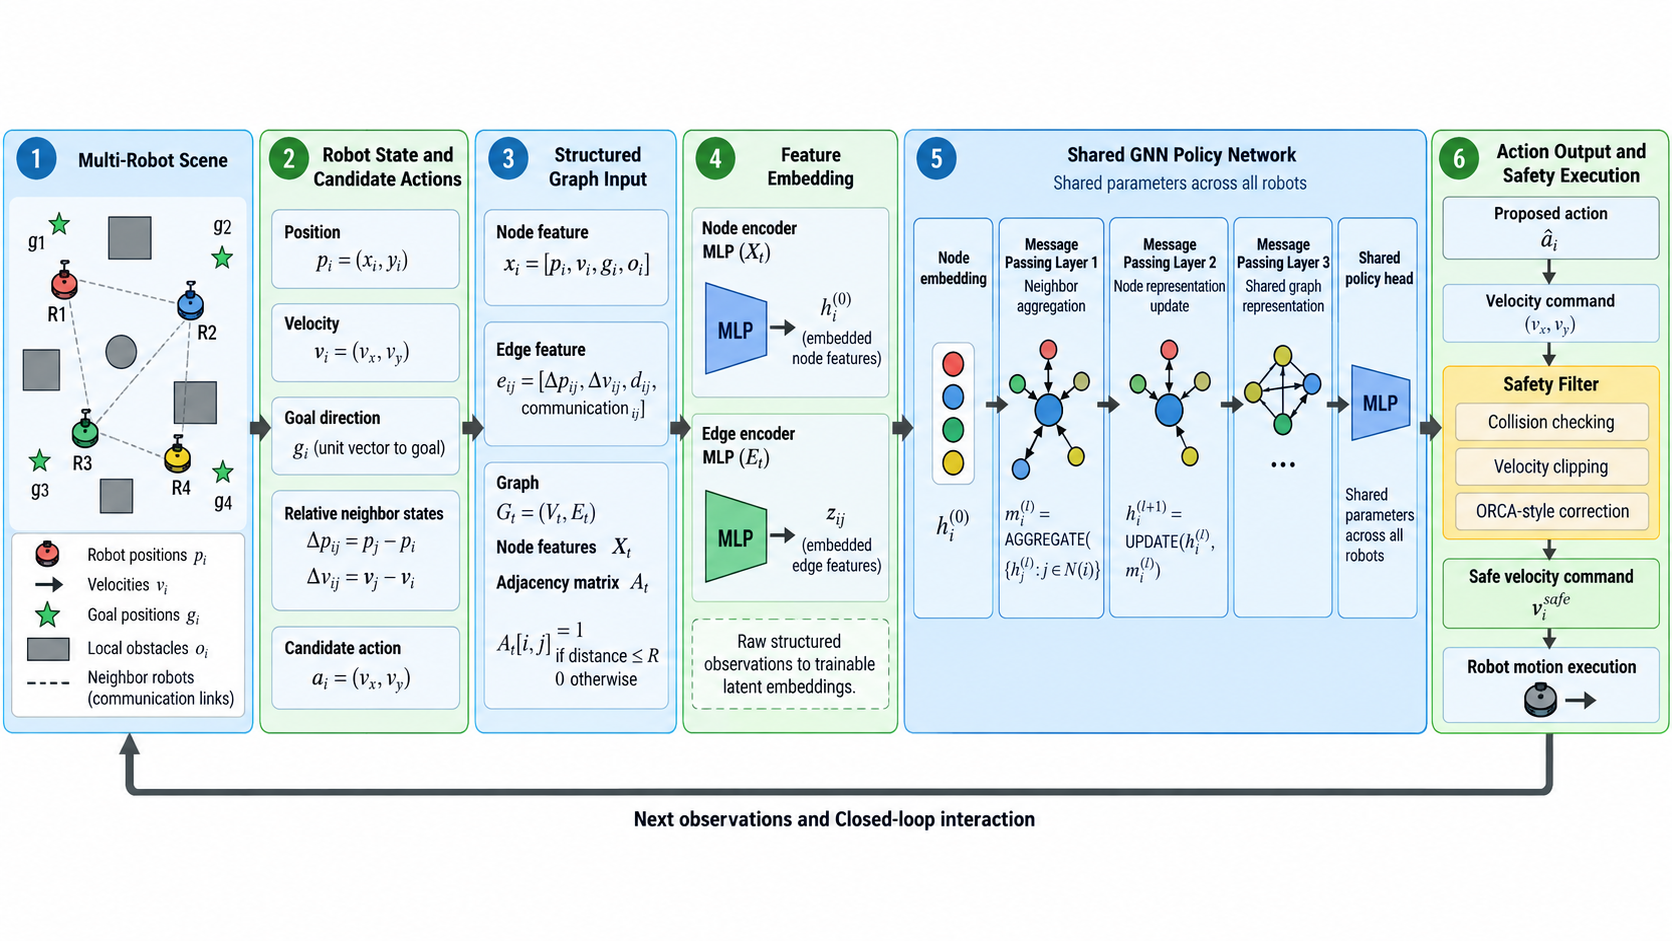
\includegraphics[width=\textwidth,trim=0 65bp 0 85bp,clip]{gnn_architecture_ai_fig1_draft_v2.png}
\caption{Multi-robot navigation pipeline: robot scene and states, structured
graph inputs, feature embedding, shared GNN inference, and action output with
optional safety filtering. Executed motion closes the observation--action loop.}
\label{fig:arch}
\end{figure*}

\subsection{Baselines}
The baselines include A* grid tracking, an ORCA-style local repulsion
controller, and an RVO-style controller that samples a finite lattice of
headings and speeds. The RVO-style controller scores candidate velocities by
predicted neighbor clearance, obstacle occupancy, and goal progress. It is
implemented for this benchmark and is not a formally verified RVO reference
implementation. The independent MLP shares parameters across robots but uses
only node features, without the adjacency matrix.

\subsection{Message-Passing Policy}
A linear layer first maps node features to a hidden representation. Each
layer averages neighbor representations and updates the node from its own
state concatenated with the transformed neighborhood message:
\begin{equation}
m_i^{(l)}=\tfrac{1}{\max(1,d_i)}{\textstyle\sum_j}A_{ij}h_j^{(l)},\;
h_i^{(l+1)}=\sigma(W_l[h_i^{(l)}\Vert\phi_l(m_i^{(l)})]).
\end{equation}
With edge features the message becomes
\begin{equation}
m_i^{(l)}=\tfrac{1}{\max(1,d_i)}{\textstyle\sum_j}A_{ij}(\phi_l(h_j^{(l)})+\psi_l(e_{ij})),
\end{equation}
followed by
$h_i^{(l+1)}=\mathrm{ReLU}(W_l[h_i^{(l)}\Vert m_i^{(l)}])$. We use three
message-passing layers, 128 hidden units, and a shared action head, with the
action bounded by $\hat{u}_i=v_{\max}\tanh(f_\theta(h_i))$.

\subsection{Attention Variants}
Two attention models are evaluated with the same inputs, outputs, data,
and test scenarios. The neighbor-attention GNN replaces mean aggregation
with multi-head attention over queries, keys, and values, masked by the local
adjacency. The graph transformer uses adjacency-masked multi-head
self-attention, residual connections, and feed-forward blocks. Both models
use 128 hidden units, four heads, and a shared policy head.

\subsection{Training Objective}
Pure action imitation reproduces the expert's local behavior but does not
guarantee a safe closed loop, so we train on a weighted sum of four terms:
\begin{equation}
\mathcal{L}=\lambda_a\mathcal{L}_{act}+\lambda_c\mathcal{L}_{col}
+\lambda_p\mathcal{L}_{prog}+\lambda_s\mathcal{L}_{smooth},
\end{equation}
where $\mathcal{L}_{act}=\frac{1}{|\mathcal{V}|}\sum_i
\mathrm{Huber}(u_i,u_i^*)$ is the imitation term. Writing the one-step
predicted pair distance as $d_{ij}'=\|p_i+\Delta t\,u_i-p_j-\Delta t\,u_j\|$,
$\mathcal{L}_{col}=\frac{1}{N(N-1)}\sum_{i\neq j}[d_s-d_{ij}']_+^2$ penalizes
predicted distances below the safety threshold. The remaining terms are
\begin{equation}
\begin{aligned}
\mathcal{L}_{prog}&=\tfrac{1}{N}{\textstyle\sum_i}[\|g_i-p_i'\|-\|g_i-p_i\|]_+,\\
\mathcal{L}_{smooth}&=\tfrac{1}{N}{\textstyle\sum_i}\|u_i^t-u_i^{t-1}\|_2^2,
\end{aligned}
\end{equation}
with $[x]_+=\max(x,0)$. Padding nodes are masked by $q_i\in\{0,1\}$, so every
node loss becomes $\sum_i q_i\ell_i/\max(1,\sum_i q_i)$ and a graph padded to
40 nodes trains on exactly the real robots in it.

Multi-scale training samples datasets with 5--40 robots from all four map
families and pads each graph to 40 nodes. The progress term penalizes motion
away from the goal, while the smoothness term limits changes between
successive actions.

\subsection{Safety Filter}
After the policy emits its action, the filter inspects every close pair and
applies a symmetric correction before clipping. Let
$n_{ij}=\delta_{ij}/(\|\delta_{ij}\|+\epsilon)$ with $\delta_{ij}=p_i-p_j$. If
$\|\delta_{ij}\|<d_s+\tau$ and $(u_i-u_j)\cdot n_{ij}<0$, then
\begin{equation}
\begin{aligned}
\tilde{u}_i&=u_i+\tfrac{\kappa_{ij}}{2}n_{ij},\quad
\tilde{u}_j=u_j-\tfrac{\kappa_{ij}}{2}n_{ij},\\
\kappa_{ij}&=-(u_i-u_j)\cdot n_{ij}+[d_s+\tau-\|\delta_{ij}\|]_+,
\end{aligned}
\end{equation}
after which each $\tilde{u}_i$ is clipped to $v_{\max}$. The filter operates
only during inference; Section~\ref{sec:results} evaluates its effect
separately from that of the learned policy.

\section{Experimental Setup}

Experiments span four map families---\textit{crossing}, \textit{open},
\textit{random}, and \textit{narrow}---and 5, 10, 20, 30, and 40 robots.
Development data uses fixed seeds with 20 episodes of at most 160 steps each.
The main evaluation covers $4\times3\times5\times10=600$ episodes over
three robot counts, five methods, and ten fixed test seeds; the extended
learned-model comparison covers 480 episodes for four learned policies; and
the multi-scale test covers 1800 safety-filtered and 1800 unfiltered episodes
over 30 unseen seeds (100--129). All methods share initial states, goals,
obstacles, action limits, and termination rules. Data are stored as compressed
NPZ archives holding features, adjacency, actions, positions, rewards,
obstacles, layout, expert identifier, and step index.

Reported metrics are goal success rate, strict no-physical-collision success
rate, safety-violation events, physical collision events, minimum inter-robot
separation, path length, final goal error, and mean per-step control time.
Means, standard deviations, and 95\% confidence intervals are computed over
episodes, and violations at $0.72$~m and physical collisions at $0.56$~m are
always reported in separate columns. Training used one 24~GB GPU with batch
size 128.

\section{Results}
\label{sec:results}

\subsection{Main Comparison}
Table~\ref{tab:main} summarizes the 600-episode main comparison. A* attains
a task success rate of 1.000 at each team size. RVO-style achieves
0.975--1.000 success and the shortest paths, while its mean control time
increases from 7.8~ms at 5 robots to 87.4~ms at 20 robots, approximately an
11-fold increase. ORCA-style has the lowest control time and the largest
minimum separation at each team size. Among the learned policies in this
comparison, the independent MLP achieves the higher success rates
(0.725--0.875).

The mean-aggregation GNN reaches success rates of 0.625, 0.725, and 0.700
at 5, 10, and 20 robots. These rates are below those of the MLP, while the
GNN has larger minimum inter-robot separation at each team size. The GNN
checkpoint was trained only on 10-robot data; its 5- and 20-robot results
therefore measure generalization across team sizes. The graph ablation below
compares the same network with and without communication edges to isolate
the effect of message passing.

\begin{table*}[t]
\caption{Main comparison over four map families and ten fixed test seeds
(40 episodes per cell). Succ: goal success. Coll: collision events, counting
transitions into a $<0.72$~m safety violation. Sep: minimum inter-robot
separation (m). $T$: mean per-step control time (ms).}
\label{tab:main}
\centering
\scriptsize
\setlength{\tabcolsep}{3pt}
\begin{tabular}{lcccccccccccc}
\toprule
& \multicolumn{4}{c}{5 robots} & \multicolumn{4}{c}{10 robots} & \multicolumn{4}{c}{20 robots}\\
\cmidrule(lr){2-5}\cmidrule(lr){6-9}\cmidrule(lr){10-13}
Method & Succ & Coll & Sep & $T$ & Succ & Coll & Sep & $T$ & Succ & Coll & Sep & $T$\\
\midrule
A*         & 1.000 & 1.925  & 0.280 & 0.512 & 1.000 & 6.075  & 0.098 & 1.205 & 1.000 & 30.700 & 0.035 & 2.493\\
ORCA-style & 0.775 & 1.425  & 0.396 & 0.213 & 0.825 & 3.825  & 0.296 & 0.486 & 0.825 & 13.500 & 0.230 & 1.303\\
RVO-style  & 0.975 & 1.825  & 0.294 & 7.779 & 1.000 & 5.575  & 0.131 & 24.941 & 1.000 & 23.325 & 0.062 & 87.373\\
MLP        & 0.725 & 2.575  & 0.191 & 0.342 & 0.850 & 5.400  & 0.095 & 0.483 & 0.875 & 27.400 & 0.038 & 0.775\\
GNN        & 0.625 & 1.850  & 0.224 & 0.683 & 0.725 & 5.675  & 0.149 & 0.828 & 0.700 & 28.675 & 0.041 & 1.129\\
\bottomrule
\end{tabular}
\end{table*}

\subsection{Attention and Transformer Variants}
Table~\ref{tab:learned} compares four learned policies over 480 episodes.
Goal success is 0.817 for the MLP, 0.683 for the GNN, 0.558 for the graph
transformer, and 0.342 for the neighbor-attention GNN. Their strict
collision-free success rates are 0.017, 0.008, 0.058, and 0.025,
respectively. The graph transformer has the highest strict success rate,
with a mean control time of 1.365~ms compared with 0.856~ms for the GNN.
Neighbor attention increases mean minimum separation to 0.259~m, but lowers
goal success and takes 1.298~ms per step. These unfiltered policies remain
insufficient for reliable collision-free navigation.

\begin{table}[t]
\caption{Learned-policy comparison (480 episodes). Strict success requires
goal arrival with no pair ever closer than the 0.56~m physical diameter.}
\label{tab:learned}
\centering
\footnotesize
\setlength{\tabcolsep}{3.5pt}
\begin{tabular}{lrrrrr}
\toprule
Model & Success & Strict & Phys.\ coll. & Min.\ sep. & Time\\
      &         & succ.  & events      & (m)        & (ms)\\
\midrule
MLP               & 0.817 & 0.017 & 9.250 & 0.108 & 0.515 \\
GNN               & 0.683 & 0.008 & 8.825 & 0.138 & 0.856 \\
Neighbor-attention & 0.342 & 0.025 & 8.167 & 0.259 & 1.298 \\
Graph transformer & 0.558 & 0.058 & 8.833 & 0.221 & 1.365 \\
\bottomrule
\end{tabular}
\end{table}

\begin{figure}[t]
\centering
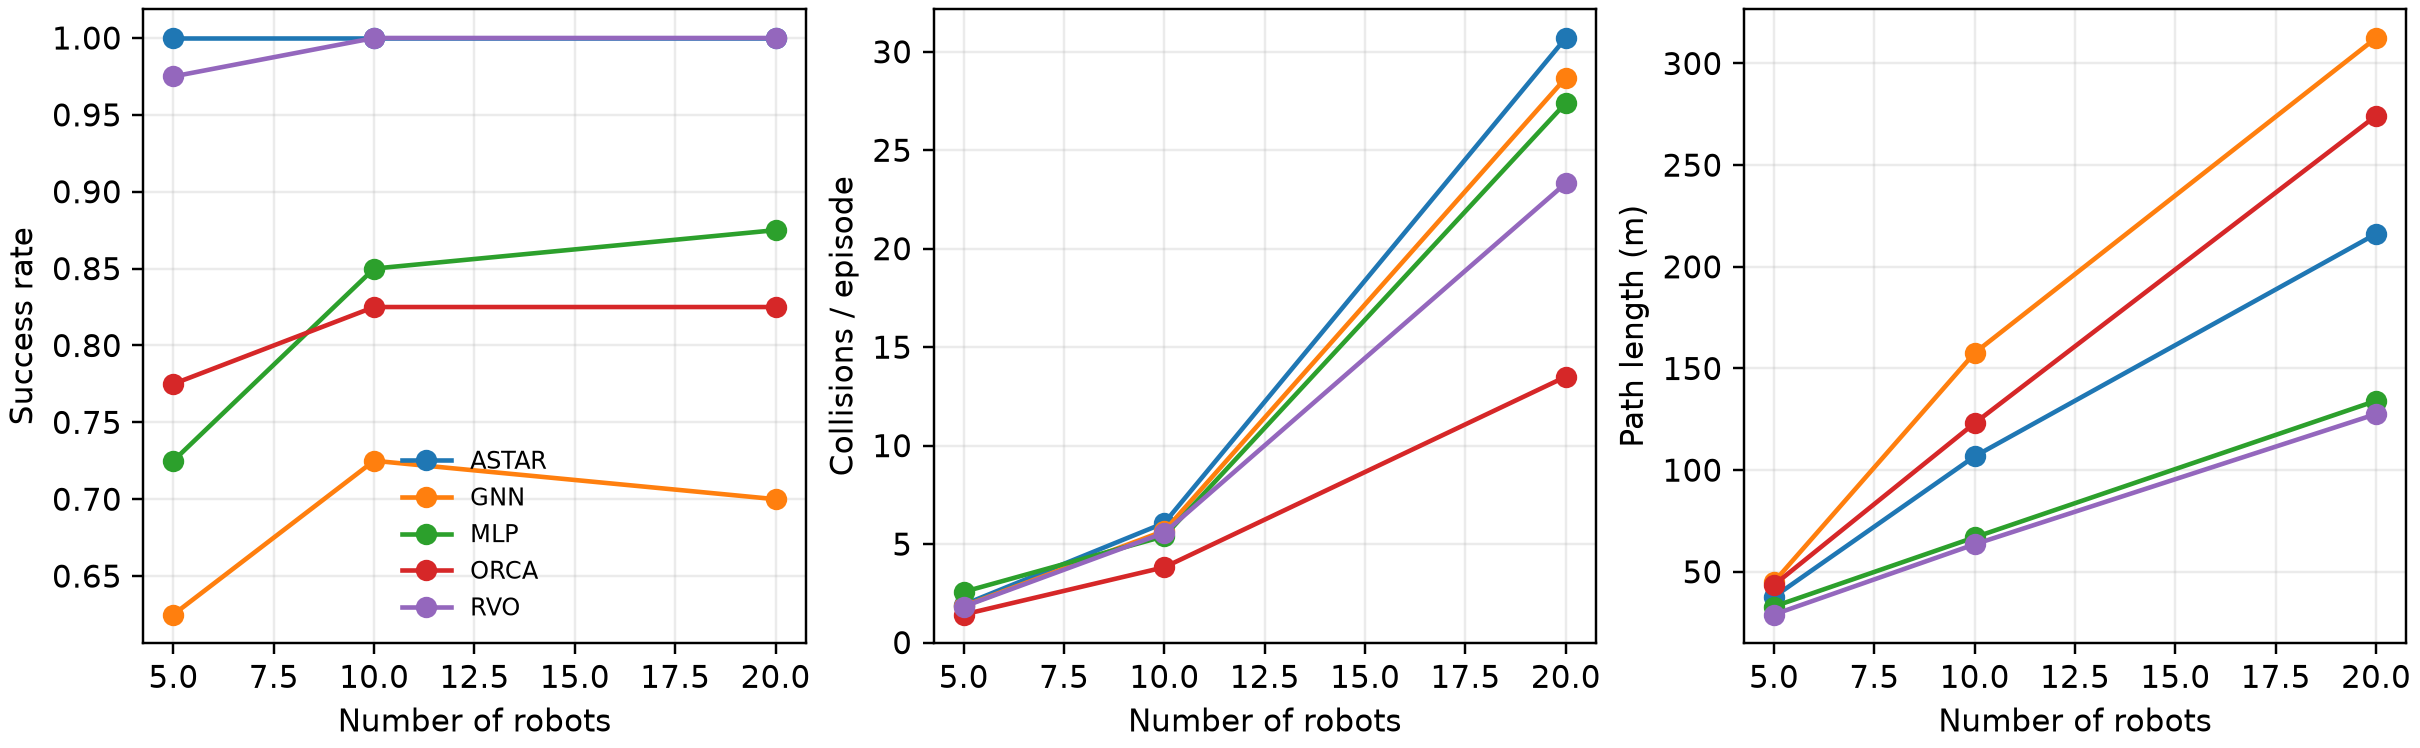
\includegraphics[width=\columnwidth]{baselines_final.png}
\caption{Comparison of goal success, path length, and control time across methods
and team sizes in the 600-episode main evaluation.}
\label{fig:baselines}
\end{figure}

\subsection{Graph Structure Ablation}
The graph ablation compares local, global, and edge-free connectivity
(Fig.~\ref{fig:ablations}a). At 10 robots, the local graph reaches 0.725
success compared with 0.425 for the edge-free policy of the same capacity,
an increase of 30 percentage points. At 5 and 20 robots, the corresponding
increases are 12.5 and 27.5 percentage points. Fully connecting the graph
does not improve on local communication; at 10 robots, success is 0.625 for
the global graph and 0.725 for the local graph. These results support local
neighbor exchange for goal reaching, although collisions remain in both
graph variants.

\subsection{Safety Filter Ablation}
The safety-filter ablation compares raw and corrected GNN actions over 60
episodes (Fig.~\ref{fig:ablations}b). At 10 robots, filtering reduces mean
safety-violation events from 4.900 to 0.200 and increases mean minimum
separation from 0.069~m to 0.794~m, while goal success decreases from 1.000
to 0.900. At 20 robots, violation events decrease from 27.500 to 6.900 and
goal success from 0.900 to 0.700; mean minimum separation is 0.067~m.
The correction improves spacing but can impede goal progress. Its limited
effect at 20 robots motivates further study of safety constraints during
training.

\begin{figure*}[t]
\centering
\begin{minipage}[t]{0.49\textwidth}
\centering
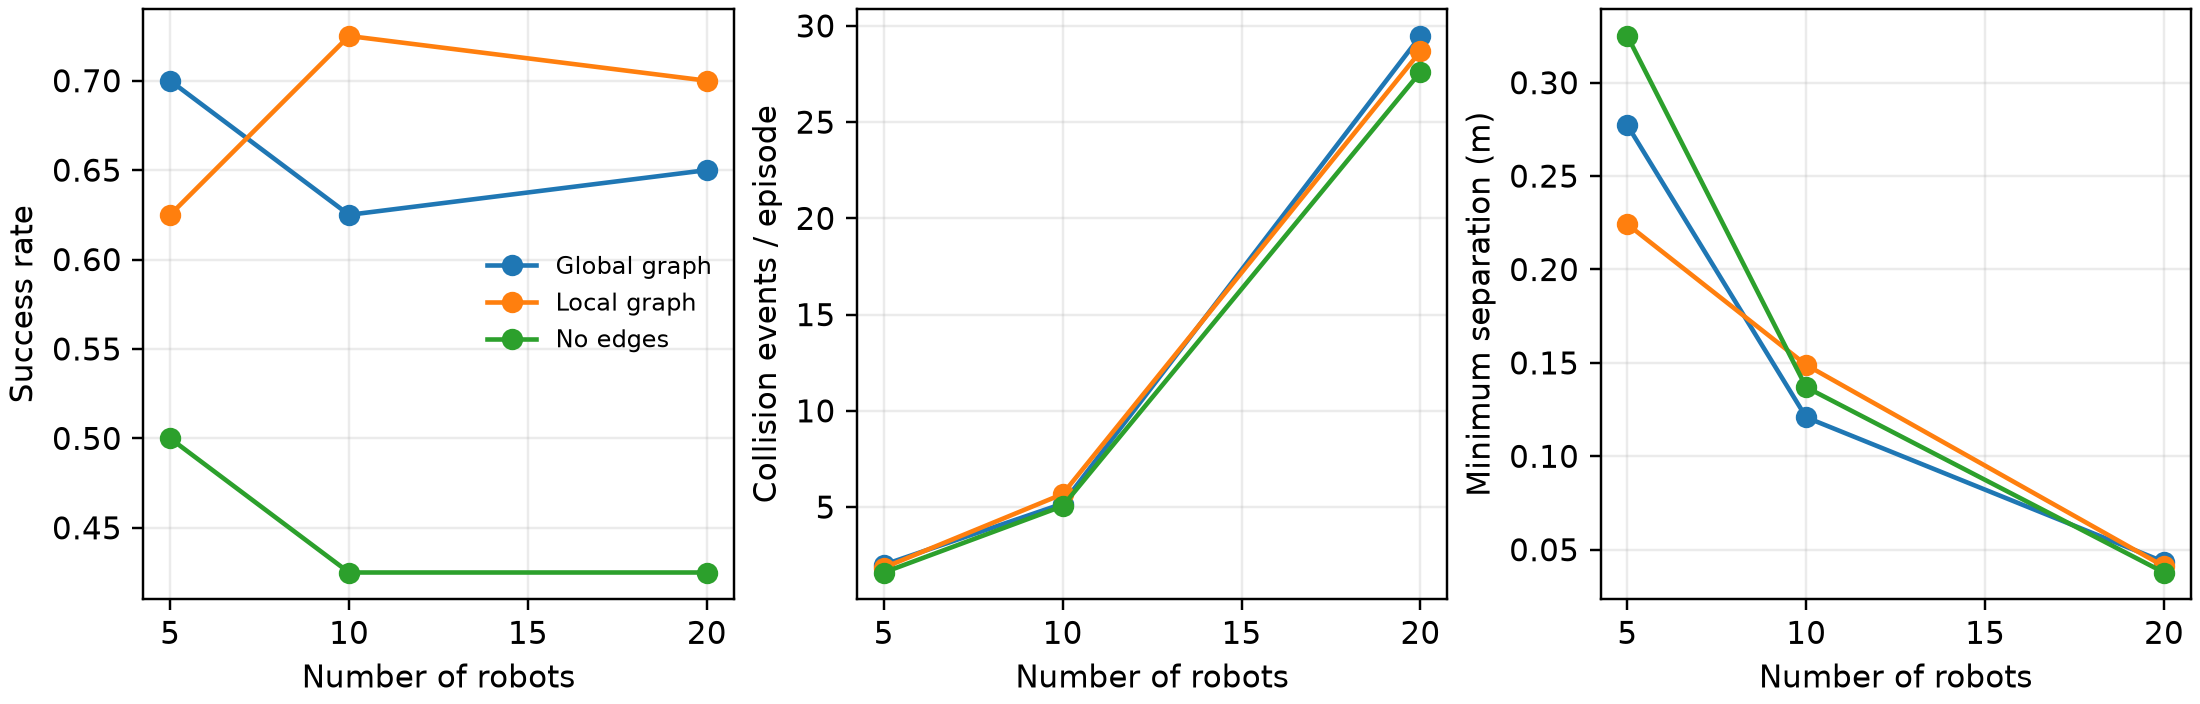
\includegraphics[width=\linewidth]{ablation_graph_final.png}\\
(a) Graph structure
\end{minipage}\hfill
\begin{minipage}[t]{0.49\textwidth}
\centering
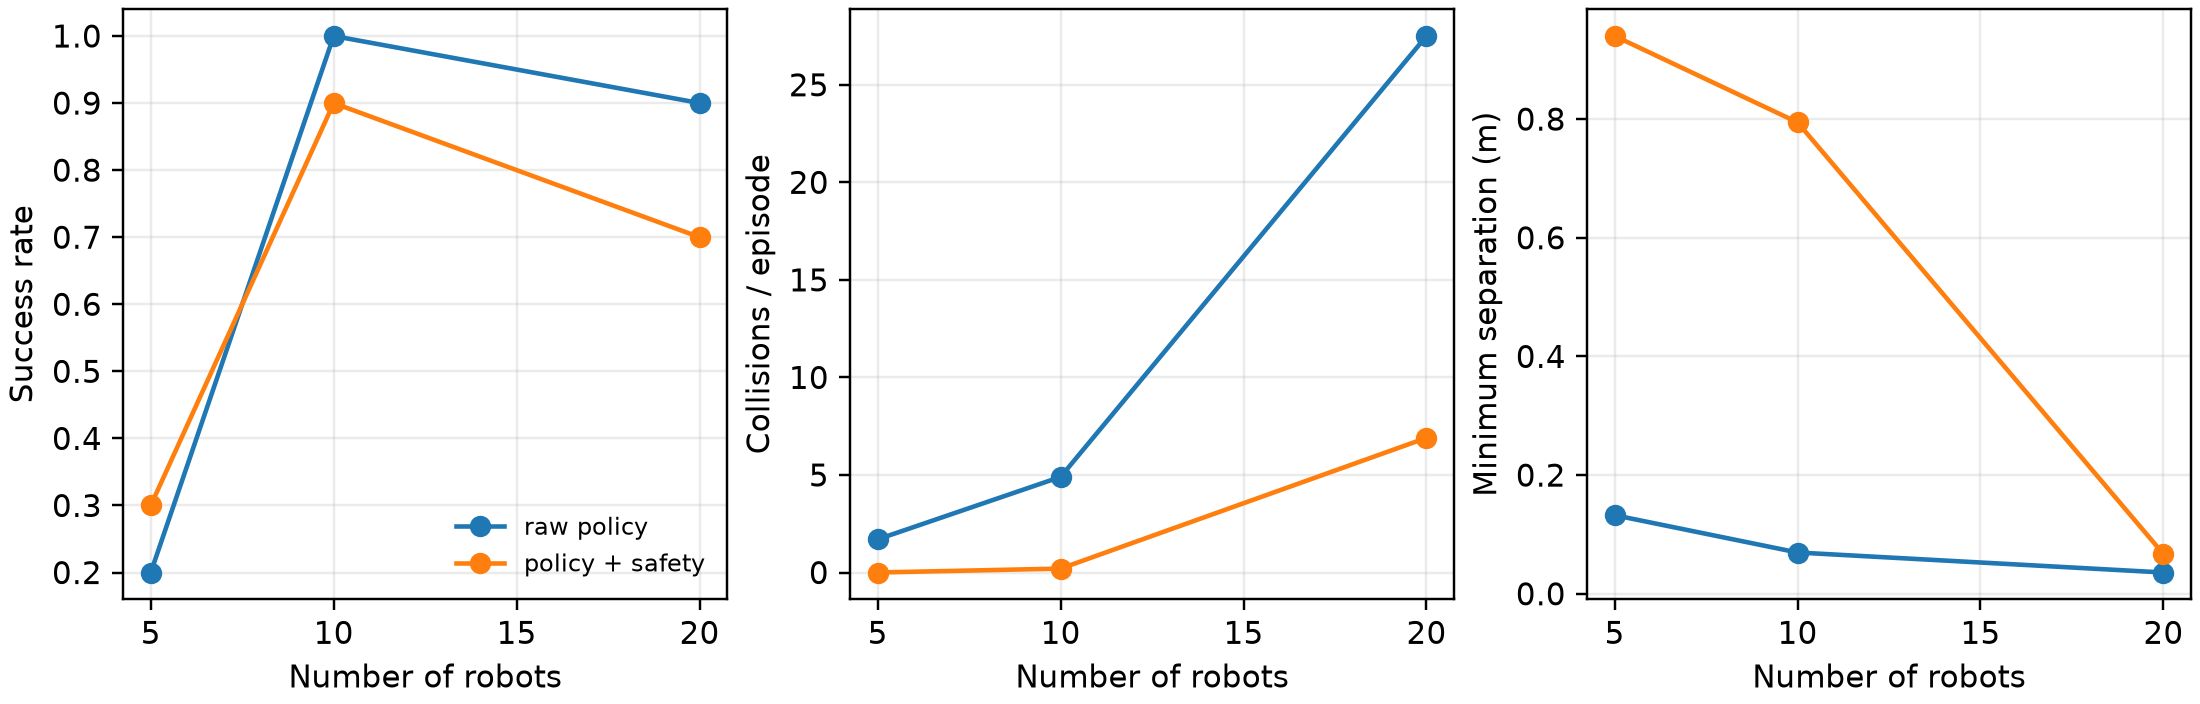
\includegraphics[width=\linewidth]{ablation_safety_final.png}\\
(b) Safety filter
\end{minipage}
\caption{Ablation results at 5, 10, and 20 robots. (a) Goal success with edge-free,
local, and global graphs. (b) Goal success, safety-violation events, and
minimum separation before and after safety filtering.}
\label{fig:ablations}
\end{figure*}

\subsection{Communication Radius}
Increasing the communication radius adds neighbors to each robot's graph.
At 10 robots, a radius of 2.0~m gives a mean degree of 0.463 and success of
0.200. Radii of 3.4~m and 5.5~m increase mean degree to 2.283 and 4.420,
respectively, and both achieve success of 1.000. The global graph has mean
degree 9.000 and success 0.900. At 5 robots, success increases from 0.100
at 2.0~m to 1.000 with the global graph. The results indicate that a small
radius can restrict information exchange, while additional neighbors beyond
an adequate local range do not consistently improve success. Control time
ranges from about 0.8 to 1.5~ms across the tested settings, and physical collisions are not
eliminated by global connectivity.

\subsection{Multi-Scale Stress Test}
Table~\ref{tab:multiscale} reports the 1800-episode safety-filtered test
using 30 unseen seeds per configuration. At 5 and 10 robots, GNN strict
collision-free success is 0.967 and 0.958, respectively, with no recorded
physical collisions. The graph transformer achieves 0.983 and 1.000 under
the same conditions. At 20 robots, goal success is 0.758 for the GNN and
0.842 for the transformer, and strict success is 0.708 and 0.767.
At 30 and 40 robots, strict success decreases to 0.250 and 0.000 for the
GNN, and to 0.242 and 0.017 for the transformer. At 40 robots, mean physical
collision events reach 6.883 for the GNN and 9.025 for the transformer, with
minimum separation near 0.4~m. GNN mean control time increases from
0.890~ms at 5 robots to 2.066~ms at 40 robots.

Without filtering, the GNN achieves goal success of 0.975--1.000 across
team sizes, but strict collision-free success is 0.092 at 5 robots and
0.000 at larger sizes. The unfiltered transformer's strict success does
not exceed 0.117. Filtering therefore improves collision-free arrival,
particularly at 5--10 robots, while reducing goal-reaching success. At
30--40 robots, both completion and safety deteriorate in the filtered
policies, limiting their use at these densities.

\begin{table}[t]
\caption{Multi-scale test with the safety filter over 30 unseen seeds
(1800 episodes), aggregated over four map families and indexed by robot
count. Strict success requires goal arrival with no physical collision.}
\label{tab:multiscale}
\centering
\footnotesize
\setlength{\tabcolsep}{4pt}
\resizebox{\columnwidth}{!}{%
\begin{tabular}{lccccc}
\toprule
Model & 5 & 10 & 20 & 30 & 40\\
\midrule
\multicolumn{6}{l}{\textit{Goal success / strict collision-free success}}\\
GNN      & 0.967/0.967 & 0.958/0.958 & 0.758/0.708 & 0.400/0.250 & 0.042/0.000\\
Transformer & 0.983/0.983 & 1.000/1.000 & 0.842/0.767 & 0.467/0.242 & 0.108/0.017\\
\addlinespace
\multicolumn{6}{l}{\textit{Physical collision events per episode}}\\
GNN      & 0.000 & 0.000 & 0.075 & 1.158 & 6.883\\
Transformer & 0.000 & 0.000 & 0.217 & 2.267 & 9.025\\
\addlinespace
\multicolumn{6}{l}{\textit{Minimum separation (m) / control time (ms)}}\\
GNN      & 0.97/0.89 & 0.95/1.04 & 0.87/1.37 & 0.61/1.70 & 0.41/2.07\\
Transformer & 1.00/1.50 & 0.94/1.65 & 0.80/1.99 & 0.56/2.33 & 0.34/2.69\\
\bottomrule
\end{tabular}}
\end{table}

\begin{figure}[t]
\centering
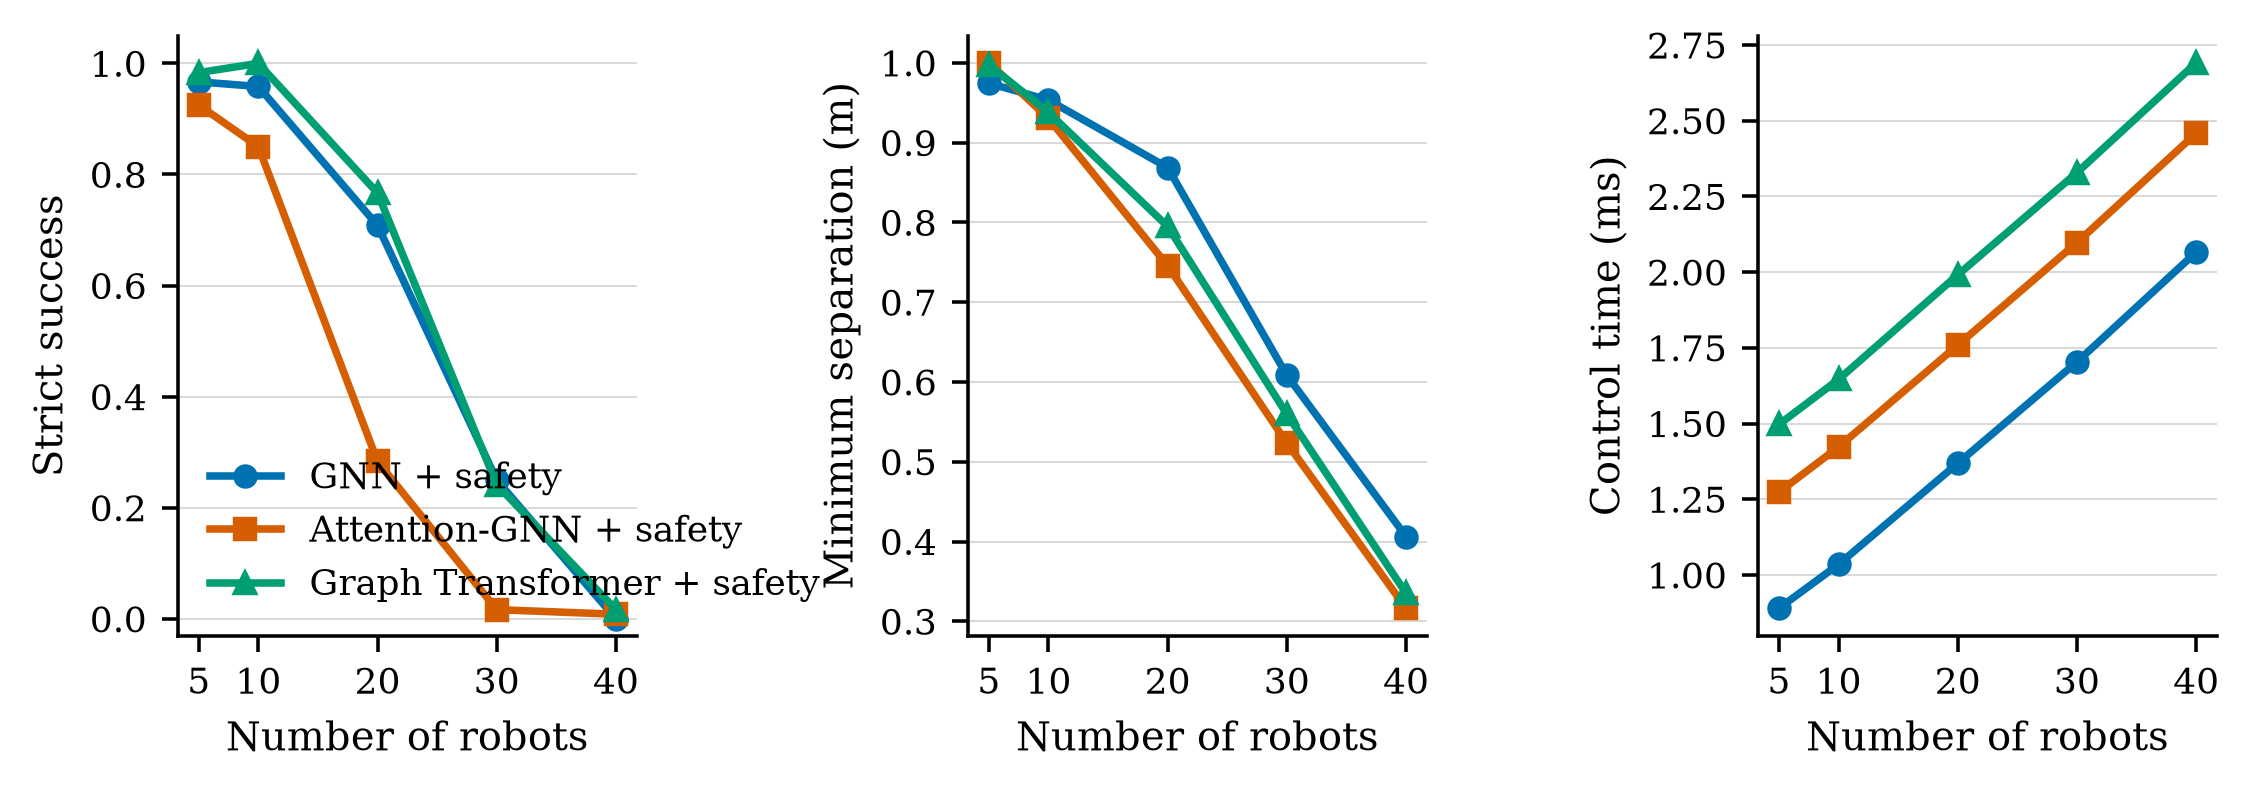
\includegraphics[width=\columnwidth]{multiscale_safety_scaling.png}
\caption{Strict collision-free success, minimum separation, and mean control time
with safety filtering at different team sizes. Collision-free success
decreases as the number of robots exceeds 20.}
\label{fig:scaling}
\end{figure}

\begin{figure*}[t]
\centering
\begin{minipage}[t]{0.30\textwidth}
\centering
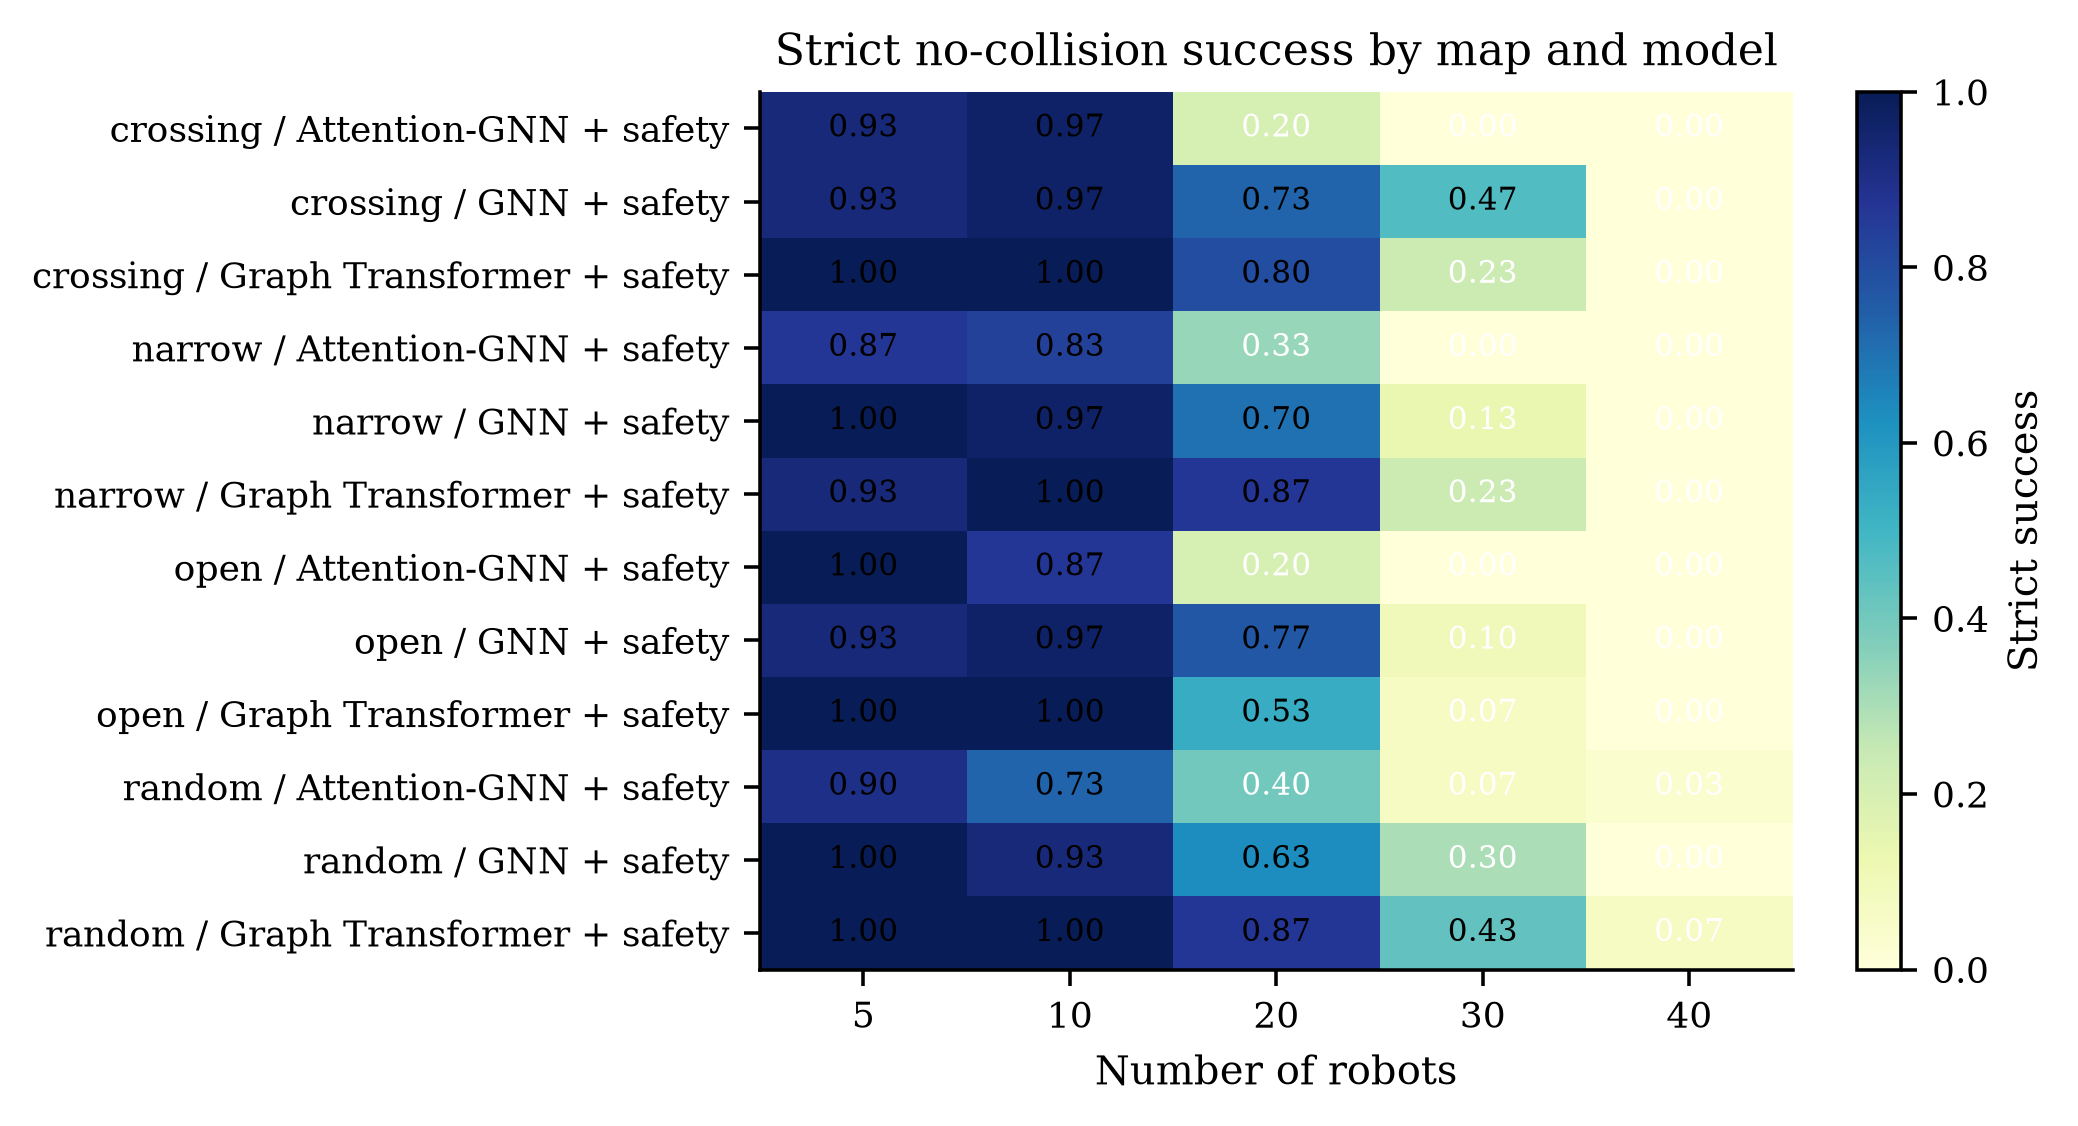
\includegraphics[width=\linewidth]{multiscale_map_heatmap.png}\\
(a) Strict success by map and density
\end{minipage}\hfill
\begin{minipage}[t]{0.68\textwidth}
\centering
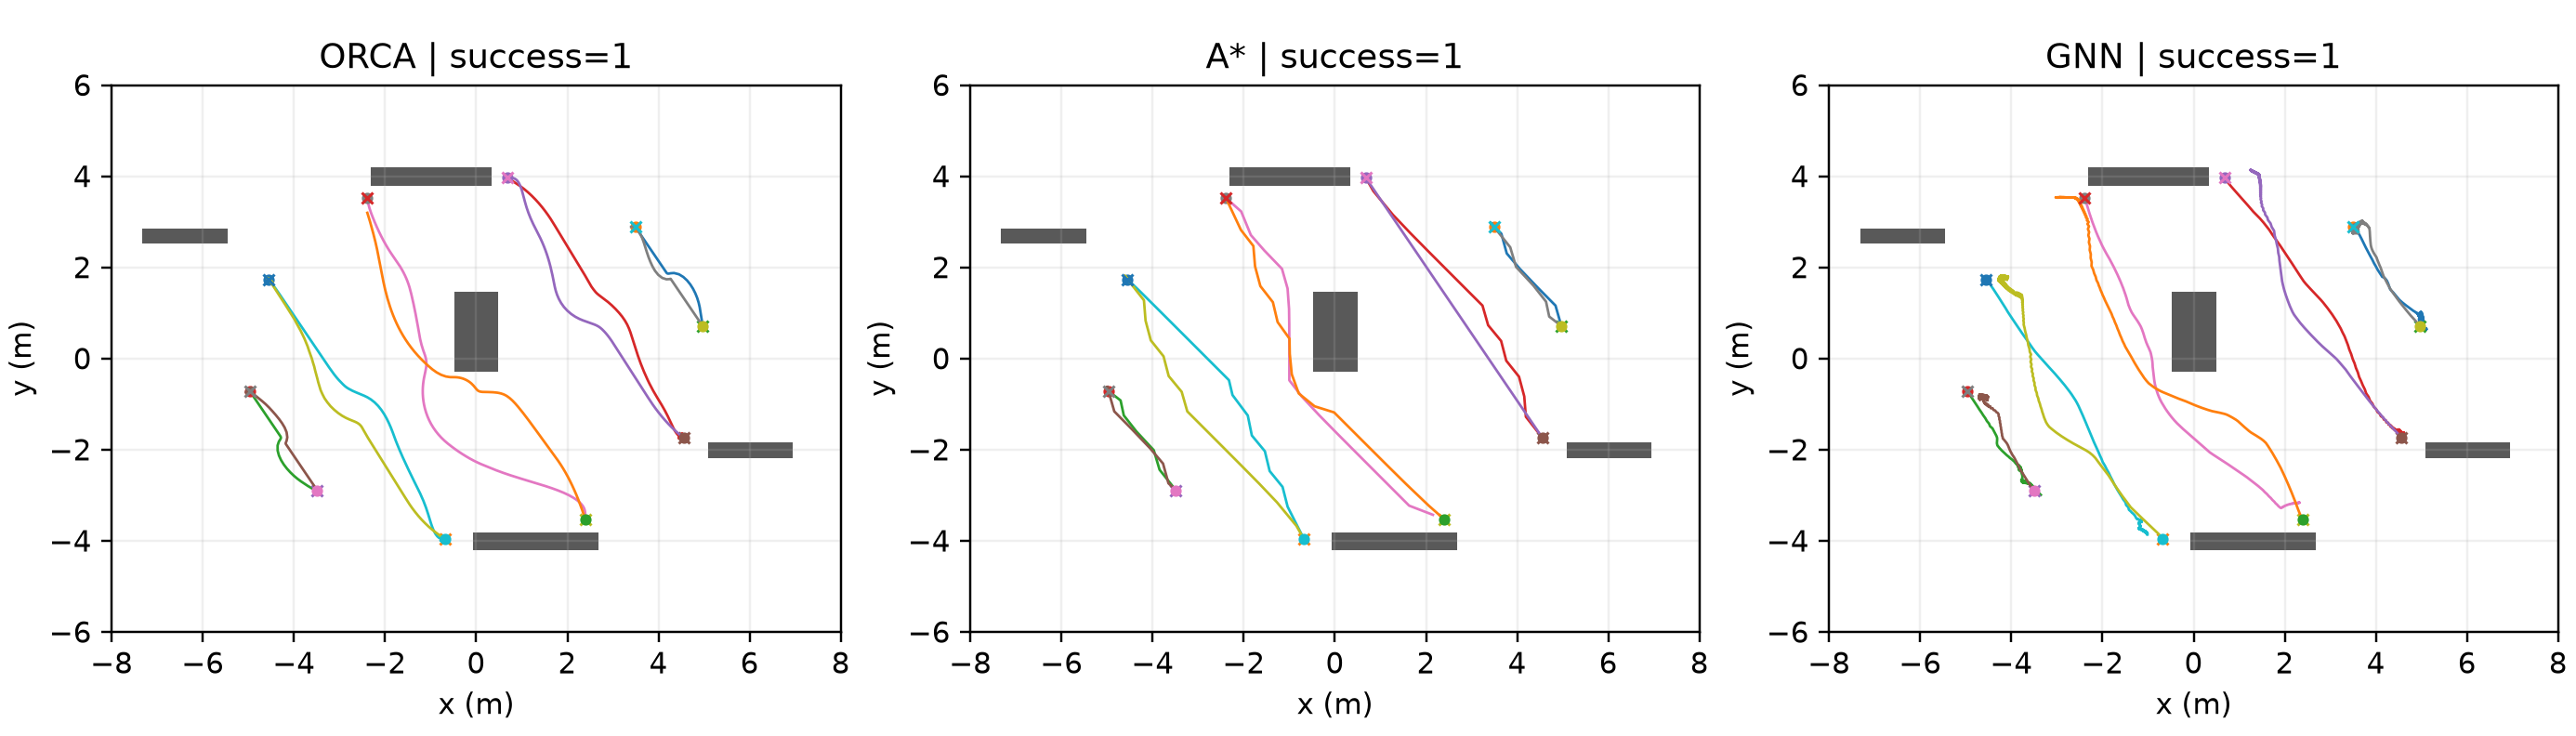
\includegraphics[width=\linewidth]{trajectories_final.png}\\
(b) Representative trajectories
\end{minipage}
\caption{(a) Strict collision-free success by map family and population size;
\textit{random} and \textit{narrow} layouts are the most demanding at high
density. (b) Representative trajectories, with communication edges drawn as
transient links between robots within the radius.}
\label{fig:mapstraj}
\end{figure*}

\subsection{Seed Stability}
Three independently trained GNN checkpoints give mean success of
$0.517\pm0.388$, $0.767\pm0.161$, and $0.850\pm0.115$ at 5, 10, and 20 robots.
The standard deviations are computed across checkpoint-level mean success
rates. Variation is largest at 5 robots, indicating sensitivity to the
training seed in this setting. This analysis evaluates training variability
separately from the episode-level averages reported for fixed checkpoints
in the preceding comparisons.

\section{Limitations and Conclusion}

This paper presents a dynamic graph policy for multi-robot navigation with
relative-motion edge features, a joint imitation objective, and an external
safety filter. Local message passing improves goal success relative to an
edge-free policy of the same capacity, while global connectivity offers no
consistent additional benefit. Safety filtering increases inter-robot
separation and supports high collision-free success at 5--10 robots in the
multi-scale test. The GNN maintains millisecond-level control time across
the tested team sizes.

The experiments also identify limits. The mean-aggregation GNN does not
exceed the independent MLP's goal success in the main comparison, and strict
collision-free success declines at 30--40 robots. The main GNN checkpoint is
trained at one team size, and the rule-based expert constrains the behaviors
available for imitation. The RVO-style baseline uses finite candidate
sampling and should not be equated with a verified RVO implementation.
Evaluation is limited to simulation. Further work will examine training
with explicit safety constraints, comparison with reference RVO
implementations, cross-map generalization, and physical-robot experiments.

% The IEEEtran bibliography defaults to \footnotesize; tighten it slightly so
% the reference list fits the six-page limit without dropping citations.
\renewcommand{\footnotesize}{\fontsize{7.5}{8.6}\selectfont}
\bibliographystyle{IEEEtran}
\bibliography{references}

\end{document}
